\documentclass[french,]{article}
\usepackage{lmodern}
\usepackage{amssymb,amsmath}
\usepackage{ifxetex,ifluatex}
\usepackage{fixltx2e} % provides \textsubscript
\ifnum 0\ifxetex 1\fi\ifluatex 1\fi=0 % if pdftex
  \usepackage[T1]{fontenc}
  \usepackage[utf8]{inputenc}
\else % if luatex or xelatex
  \ifxetex
    \usepackage{mathspec}
  \else
    \usepackage{fontspec}
  \fi
  \defaultfontfeatures{Ligatures=TeX,Scale=MatchLowercase}
\fi
% use upquote if available, for straight quotes in verbatim environments
\IfFileExists{upquote.sty}{\usepackage{upquote}}{}
% use microtype if available
\IfFileExists{microtype.sty}{%
\usepackage{microtype}
\UseMicrotypeSet[protrusion]{basicmath} % disable protrusion for tt fonts
}{}
\usepackage{hyperref}
\hypersetup{unicode=true,
            pdftitle={Rapport TP3 - Design Pattern},
            pdfauthor={Fleury Malik - malik.fleury@he-arc.ch; Wermeille Bastien - bastien.wermeille@he-arc.ch; Bulloni Lucas - lucas.bulloni@he-arc.ch},
            pdfborder={0 0 0},
            breaklinks=true}
\urlstyle{same}  % don't use monospace font for urls
\ifnum 0\ifxetex 1\fi\ifluatex 1\fi=0 % if pdftex
  \usepackage[shorthands=off,main=french]{babel}
\else
  \usepackage{polyglossia}
  \setmainlanguage[]{french}
\fi
\usepackage[top=4cm, bottom=4cm, left=4cm, right=4cm]{geometry}
\usepackage{color}
\usepackage{fancyvrb}
\newcommand{\VerbBar}{|}
\newcommand{\VERB}{\Verb[commandchars=\\\{\}]}
\DefineVerbatimEnvironment{Highlighting}{Verbatim}{commandchars=\\\{\}}
% Add ',fontsize=\small' for more characters per line
\newenvironment{Shaded}{}{}
\newcommand{\KeywordTok}[1]{\textcolor[rgb]{0.00,0.44,0.13}{\textbf{{#1}}}}
\newcommand{\DataTypeTok}[1]{\textcolor[rgb]{0.56,0.13,0.00}{{#1}}}
\newcommand{\DecValTok}[1]{\textcolor[rgb]{0.25,0.63,0.44}{{#1}}}
\newcommand{\BaseNTok}[1]{\textcolor[rgb]{0.25,0.63,0.44}{{#1}}}
\newcommand{\FloatTok}[1]{\textcolor[rgb]{0.25,0.63,0.44}{{#1}}}
\newcommand{\ConstantTok}[1]{\textcolor[rgb]{0.53,0.00,0.00}{{#1}}}
\newcommand{\CharTok}[1]{\textcolor[rgb]{0.25,0.44,0.63}{{#1}}}
\newcommand{\SpecialCharTok}[1]{\textcolor[rgb]{0.25,0.44,0.63}{{#1}}}
\newcommand{\StringTok}[1]{\textcolor[rgb]{0.25,0.44,0.63}{{#1}}}
\newcommand{\VerbatimStringTok}[1]{\textcolor[rgb]{0.25,0.44,0.63}{{#1}}}
\newcommand{\SpecialStringTok}[1]{\textcolor[rgb]{0.73,0.40,0.53}{{#1}}}
\newcommand{\ImportTok}[1]{{#1}}
\newcommand{\CommentTok}[1]{\textcolor[rgb]{0.38,0.63,0.69}{\textit{{#1}}}}
\newcommand{\DocumentationTok}[1]{\textcolor[rgb]{0.73,0.13,0.13}{\textit{{#1}}}}
\newcommand{\AnnotationTok}[1]{\textcolor[rgb]{0.38,0.63,0.69}{\textbf{\textit{{#1}}}}}
\newcommand{\CommentVarTok}[1]{\textcolor[rgb]{0.38,0.63,0.69}{\textbf{\textit{{#1}}}}}
\newcommand{\OtherTok}[1]{\textcolor[rgb]{0.00,0.44,0.13}{{#1}}}
\newcommand{\FunctionTok}[1]{\textcolor[rgb]{0.02,0.16,0.49}{{#1}}}
\newcommand{\VariableTok}[1]{\textcolor[rgb]{0.10,0.09,0.49}{{#1}}}
\newcommand{\ControlFlowTok}[1]{\textcolor[rgb]{0.00,0.44,0.13}{\textbf{{#1}}}}
\newcommand{\OperatorTok}[1]{\textcolor[rgb]{0.40,0.40,0.40}{{#1}}}
\newcommand{\BuiltInTok}[1]{{#1}}
\newcommand{\ExtensionTok}[1]{{#1}}
\newcommand{\PreprocessorTok}[1]{\textcolor[rgb]{0.74,0.48,0.00}{{#1}}}
\newcommand{\AttributeTok}[1]{\textcolor[rgb]{0.49,0.56,0.16}{{#1}}}
\newcommand{\RegionMarkerTok}[1]{{#1}}
\newcommand{\InformationTok}[1]{\textcolor[rgb]{0.38,0.63,0.69}{\textbf{\textit{{#1}}}}}
\newcommand{\WarningTok}[1]{\textcolor[rgb]{0.38,0.63,0.69}{\textbf{\textit{{#1}}}}}
\newcommand{\AlertTok}[1]{\textcolor[rgb]{1.00,0.00,0.00}{\textbf{{#1}}}}
\newcommand{\ErrorTok}[1]{\textcolor[rgb]{1.00,0.00,0.00}{\textbf{{#1}}}}
\newcommand{\NormalTok}[1]{{#1}}
\usepackage{graphicx,grffile}
\makeatletter
\def\maxwidth{\ifdim\Gin@nat@width>\linewidth\linewidth\else\Gin@nat@width\fi}
\def\maxheight{\ifdim\Gin@nat@height>\textheight\textheight\else\Gin@nat@height\fi}
\makeatother
% Scale images if necessary, so that they will not overflow the page
% margins by default, and it is still possible to overwrite the defaults
% using explicit options in \includegraphics[width, height, ...]{}
\setkeys{Gin}{width=\maxwidth,height=\maxheight,keepaspectratio}
\IfFileExists{parskip.sty}{%
\usepackage{parskip}
}{% else
\setlength{\parindent}{0pt}
\setlength{\parskip}{6pt plus 2pt minus 1pt}
}
\setlength{\emergencystretch}{3em}  % prevent overfull lines
\providecommand{\tightlist}{%
  \setlength{\itemsep}{0pt}\setlength{\parskip}{0pt}}
\setcounter{secnumdepth}{5}
% Redefines (sub)paragraphs to behave more like sections
\ifx\paragraph\undefined\else
\let\oldparagraph\paragraph
\renewcommand{\paragraph}[1]{\oldparagraph{#1}\mbox{}}
\fi
\ifx\subparagraph\undefined\else
\let\oldsubparagraph\subparagraph
\renewcommand{\subparagraph}[1]{\oldsubparagraph{#1}\mbox{}}
\fi

\title{Rapport TP3 - Design Pattern}
\author{Fleury Malik -
\href{mailto:malik.fleury@he-arc.ch}{\nolinkurl{malik.fleury@he-arc.ch}} \and Wermeille Bastien -
\href{mailto:bastien.wermeille@he-arc.ch}{\nolinkurl{bastien.wermeille@he-arc.ch}} \and Bulloni Lucas -
\href{mailto:lucas.bulloni@he-arc.ch}{\nolinkurl{lucas.bulloni@he-arc.ch}}}
\date{\today}

\begin{document}
\maketitle

{
\setcounter{tocdepth}{5}
\tableofcontents
}
\section{TP3 - Rapport}\label{tp3---rapport}

\subsection{Introduction}\label{introduction}

Pour ce Travail Pratique, il a été demandé d'améliorer le TP n°2 afin
d'ajouter une abstract factory pour la création de Pizza.

Une Factory pour divers types de pizza était demandée : - Catania -
Margherita - Palerma - Profunghi

Les décorateurs des ingrédients supplémentaires ont été rajoutés avant
de commencer le travail sur les Factory.

\subsection{Abstract factory}\label{abstract-factory}

Abstract factory est un pattern qui permet de déléguer la construction
d'objets complexes à une autre classe.

\subsubsection{Réalisationg}\label{ruxe9alisationg}

Nous avons couplé l'implémentation de ce pattern avec le pattern Builder
que nous avions implémenté lors du TP n°2. Ce builder avait déjà été
pensé afin de simplifier la création de pizza et nécessitait qu'on lui
passe des ``Classes'' et non pas des objets.

Notre abstract factory est très bien intégrée au \texttt{Builder} ainsi,
pour créer une pizza, il suffit d'hériter de la classe
\texttt{PizzaFactory\_I} et de définir le type de pâte, la sauce et de
spécifier la liste des ingrédients que contiendra la pizza.

\paragraph{Exemple de code}\label{exemple-de-code}

Voici le code de l'\texttt{Abstract\ Factory}, son fonctionnement est
très simple.

\begin{Shaded}
\begin{Highlighting}[]
\KeywordTok{public} \KeywordTok{abstract} \KeywordTok{class} \NormalTok{PizzaFactory_A \{}

 \KeywordTok{public} \FunctionTok{PizzaFactory_A}\NormalTok{() \{}
  \NormalTok{listIngredient = }\KeywordTok{new} \NormalTok{ArrayList<>();}
 \NormalTok{\}}

 \KeywordTok{public} \NormalTok{Class<? }\KeywordTok{extends} \NormalTok{PizzaBase> }\FunctionTok{getNewThickness}\NormalTok{()\{}
  \KeywordTok{return} \NormalTok{pizza;}
 \NormalTok{\}}

 \KeywordTok{public} \NormalTok{Class<? }\KeywordTok{extends} \NormalTok{DecoratorSauce> }\FunctionTok{getNewSauce}\NormalTok{()\{}
  \KeywordTok{return} \NormalTok{sauce;}
 \NormalTok{\}}

 \KeywordTok{public} \NormalTok{List<Class<? }\KeywordTok{extends} \NormalTok{DecoratorIngredient>> }\FunctionTok{getNewIngredients}\NormalTok{()\{}
  \KeywordTok{return} \NormalTok{listIngredient;}
 \NormalTok{\}}

 \NormalTok{Class<? }\KeywordTok{extends} \NormalTok{PizzaBase> pizza;}
 \NormalTok{Class<? }\KeywordTok{extends} \NormalTok{DecoratorSauce> sauce;}
 \NormalTok{List<Class<? }\KeywordTok{extends} \NormalTok{DecoratorIngredient>> listIngredient;}
\NormalTok{\}}
\end{Highlighting}
\end{Shaded}

Voici l'implémentation d'une \texttt{concrete\ factory}, dans ce cas
Margherita.

\begin{Shaded}
\begin{Highlighting}[]
\KeywordTok{public} \KeywordTok{class} \NormalTok{PizzaFactoryMargherita }\KeywordTok{extends} \NormalTok{PizzaFactory_A\{}

 \KeywordTok{public} \FunctionTok{PizzaFactoryMargherita}\NormalTok{() \{}
  \KeywordTok{super}\NormalTok{();}
  \KeywordTok{this}\NormalTok{.}\FunctionTok{pizza} \NormalTok{= PizzaThin.}\FunctionTok{class}\NormalTok{;}
  \KeywordTok{this}\NormalTok{.}\FunctionTok{sauce} \NormalTok{= DecoratorTomato.}\FunctionTok{class}\NormalTok{;}
  \KeywordTok{this}\NormalTok{.}\FunctionTok{listIngredient}\NormalTok{.}\FunctionTok{add}\NormalTok{(DecoratorMozzarella.}\FunctionTok{class}\NormalTok{);}
  \KeywordTok{this}\NormalTok{.}\FunctionTok{listIngredient}\NormalTok{.}\FunctionTok{add}\NormalTok{(DecoratorOregano.}\FunctionTok{class}\NormalTok{);}
 \NormalTok{\}}
\NormalTok{\}}
\end{Highlighting}
\end{Shaded}

\paragraph{Diagramme de classe}\label{diagramme-de-classe}

\begin{figure}[htbp]
\centering
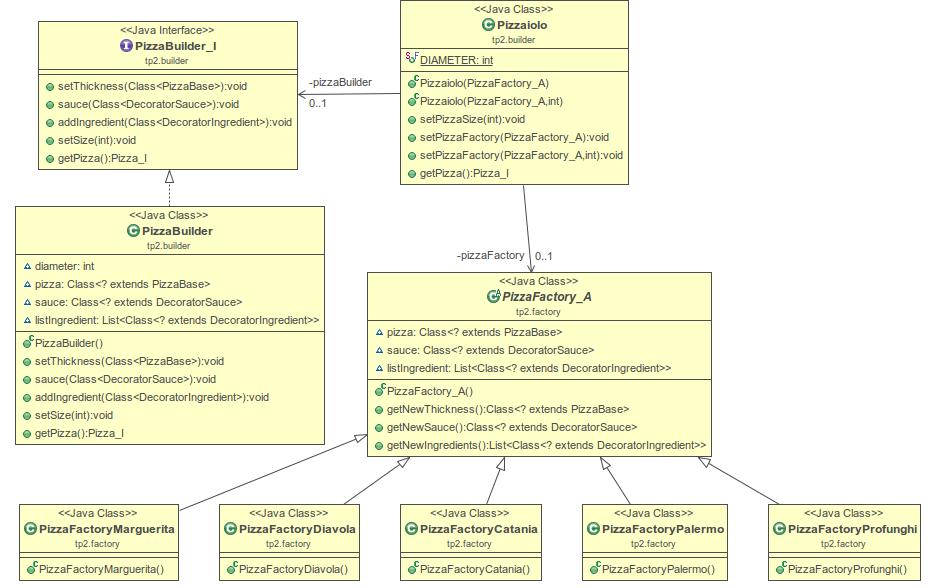
\includegraphics{factory.png}
\caption{Schema de classe}
\end{figure}


\subsubsection{Conclusion}\label{conclusion}

L'objectif est atteint. A l'aide de ce patron, nous avons la possibilité
de passer une factory à notre ``Pizzaiolo'' qui va l'utiliser afin de
réaliser de nouvelles pizzas. Ce patron s'avère très utile, car il
permet de simplifier le code du client qui va utiliser notre code pour
la création de pizza, il n'a plus à se soucier de comment la Pizza doit
être créée ni de son implémentation.

\end{document}
